\documentclass[]{article}
\usepackage{amsmath}
\usepackage{geometry}
\usepackage{enumitem}
\usepackage[colorlinks=true, urlcolor=blue]{hyperref}
\usepackage{graphicx}
\usepackage{float}
\usepackage{subfig}
\usepackage{cleveref}


\setlist{nosep}
\geometry{letterpaper, margin=1in}
%opening
\title{STAT443 Final Report}
\author{
\textbf{Group Members}\\
Nico Estrella,
Owen Kwong,
Kaichi Nakajima\\
Lily Wang,
Sky Yun
}

\begin{document}
\maketitle

\section{Summary}
Our team worked with four Canadian unemployment-related datasets to study how each factor helps us predict unemployment rates in Canada. The main goal of this project is to compare five different predictive models, including persistence, exponential, and ARIMA/ARMAX, to determine which model best predicts the unemployment rate.

In a rapidly shifting economic landscape, understanding labor market trends is critical not only from a macroeconomic perspective but also on a personal level as we prepare to transition from academia into the professional workforce. This project utilizes four distinct Canadian unemployment-related datasets to identify the underlying factors that most effectively forecast national unemployment rates. Our primary objective is to evaluate the predictive accuracy of five different forecasting models to determine the most robust framework for anticipating labor market fluctuations. By rigorously comparing these models, we aim to pinpoint the most reliable predictor of unemployment. Ultimately, this analysis grounds theoretical time series forecasting in practical reality, providing us with a data-driven understanding of the economic climate and job market we will soon be entering.

\section{Exploratory Analysis and Summary Statistics}

The main response dataset is the “Unemployment Rate Total (15-64) Canada” dataset, where the response variable is:
\vspace{0.3cm}
\begin{itemize}
\item \texttt{Unemployment}: The monthly unemployment rate (UR) of those between the ages of 15 and 64 in Canada 
\end{itemize}
\vspace{0.3cm}



The explanatory datasets consist of the total working-age population, labour-force participation rate, and interest rates. They include the following variables:


\vspace{0.3cm}
\begin{itemize}
\item \texttt{Work\_pop}: The monthly working-age population (WAP) in Canada
\item \texttt{Labor\_part}: The Canadian monthly labour-force participation (LFP) rate 
\item \texttt{Int\_rates}: Monthly Canadian interest-rate (IR)
\end{itemize}
\vspace{0.3cm}

Our analysis will have the timeframe of 1976-01-01 to 2025-12-01.

\begin{table}[H]
    \centering
    \captionsetup{justification=centering,margin=2cm}
    \begin{tabular}{|c|c|c|c|c|c|c|}
    \hline
        Time Series & Min & 25\% Q & Median & 75\% Q & max &\\
    \hline\hline
    \hline
    \end{tabular}
    \caption{Summary statistics for unemployment rate, working population total, labor force participation total, and interest rate time series.
    }
\end{table}


\subsubsection*{Time Series Plot of Training Set with STL Decomposition}

\begin{figure}[h]
\centering

\includegraphics[scale=0.5]{"figs/stl-decomp.png"}
\caption{STL Decomposition of unemployment series}
\end{figure}

The time series plot of the training set (1976-2015) shows several cyclical fluctuations in unemployment rate over time. Evidence of peaks and troughs are indicators of historical economic expansion and recession in Canada; for instance, unemployment rates peaked in the early 1980s due to a global effort of tightening monetary policies to combat rising inflation percentages. Further seasonal-trend decomposition shows a stable, repeating pattern occurring approximately yearly where year-long short-term fluctuations were observed in the time series data which strongly suggests a seasonality of period 12 present in the data. The overall trend, however, is more unclear as there is no consistent upward or downward trend; as the periods of rising and falling unemployment rates vary across the time series. It suggests that the series may be non-stationary. The remainder component suggests that the data is approximately white noise, although there are large residuals that are reflective of the aforementioned economic recessions.


\subsubsection*{ACF and PACF Plots of Training Data}

\begin{figure}[H]
\centering
\subfloat[\centering hello]
{{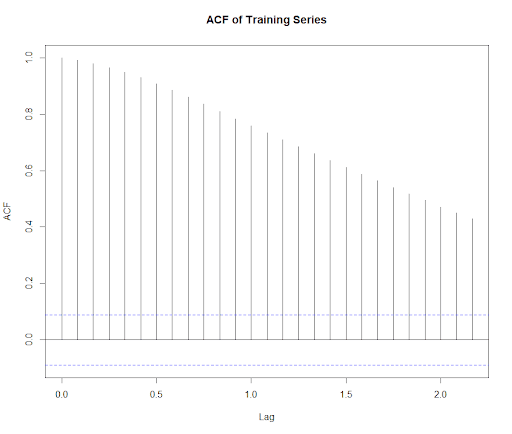
\includegraphics[width=8cm]{figs/acf-training}}}
\subfloat[\centering]
{{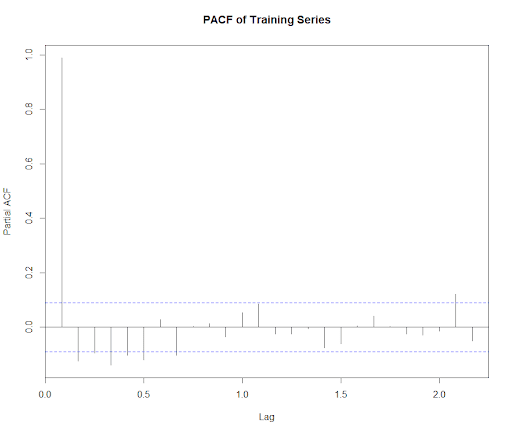
\includegraphics[width=8cm]{figs/pacf-training}}}
\caption{ACF and PACF plots for unemployment training series}
\end{figure}

Inspection of the ACF plot shows a slow decay with strong positive autocorrelations across the lags, further reinforcing the non-stationarity of the data; it may be necessary to apply first-order differencing so statistical properties such as the mean are stabilized, making it suitable for modelling using ARIMA. The PACF plot shows a cutoff directly although there are significant negative autocorrelations between lags 1-6. It suggests short-term dependence where current unemployment rates are influenced by rates within a few months ago. Therefore, the ARIMA model must also incorporate an AR component.




\section{Main Analyses and Fitted Models}


\subsection{Average Model}
\indent To establish a baseline for our forecasting, we first implemented a simple average model. This approach predicts future unemployment rates by calculating the mean of all historical observations in our training set. While computationally straightforward, this model is inherently limited because it treats all past data equally, regardless of how recently it occurred or what economic cycle it belongs to. Consequently, it yielded the highest error rate of the three models, with an \textbf{RMSE of 2.39}. The average model fails to capture the dynamic shifts, long-term trends, and repeating cycles of the Canadian economy, making it an inadequate tool for navigating the realities of the modern job market, though it serves as a necessary benchmark to prove the value of more complex forecasting methods.

\subsection{Holt-Winters Exponential Smoothing}
Moving beyond a static average, we utilized the Holt-Winters Seasonal Exponential model. This method slightly improved our predictive accuracy, reducing the \textbf{RMSE to 2.31}. The strength of Holt-Winters lies in its ability to simultaneously account for the overall level, the underlying trend, and, crucially, the seasonality of the data.

Applying a seasonal model is highly effective for unemployment data because the labor market is inherently cyclical. In Canada, employment fluctuates predictably with the seasons—for instance, retail hiring surges ahead of the winter holidays, construction and agriculture peak in the warmer months, and student employment spikes every summer. By applying exponential smoothing that weights recent seasonal patterns more heavily than older ones, the Holt-Winters model effectively anticipates these recurring macroeconomic shifts, giving us a better picture of short-term labor market health.

However, because the data has such strong cyclical patterns, the smoothing applied by Hold-Winters offers only a marginal improvement in accuracy over the average model. Despite the model applying exponential smoothing that weighs more recent patterns heavily, it still relies on averaging across multiple past periods, which introduces approximation error as it can dilute the more relevant short-term seasonal patterns. This conclusion is further supported by the persistence model, which only uses the unemployment rate from the same month of the previous year, having a better accuracy than the Holt-Winters model.

\subsection{Modified (Seasonal) Persistence Model}

Our most accurate forecast among the three came from a modified persistence model, which achieved an impressive \textbf{RMSE of approximately 2.16}. A standard persistence model (often called a "naive" forecast) simply assumes that tomorrow will be exactly like today. However, knowing that the labor market is deeply seasonal, we modified this approach to a seasonal persistence model. Instead of comparing a month to the immediately preceding month, this model predicts that a given month's unemployment rate will be identical to the rate from that exact same month in the previous year.

This model outperformed the others because it perfectly isolates the strongest driver of short-term unemployment volatility: annual cyclicality. By comparing October to last October, or May to last May, it naturally bypasses the noise of month-to-month seasonal transitions. For new graduates entering the workforce, this model underscores a vital economic reality: the most reliable indicator of what the job market will look like next month is what it looked like at this exact point in the annual cycle last year.


\subsection{ARIMA Model}

For the initial model, \texttt{auto.arima()} was used on the training set to determine the optimal model based on the lowest AIC. The model selected by this function serves as the baseline model; however, since the model with the lowest AIC does not always correspond with the best model for out-of-sample 1-step forecasts, further model selection analysis was conducted by perturbing the orders p, q, P, and Q around the baseline model using \texttt{Arima()} and then evaluating holdout set RMSE using moving 1-step forecasts.

\begin{table}[H]
    \centering
    \captionsetup{justification=centering,margin=2cm}
    \begin{tabular}{|c|c|c|}
    \hline
        Model & AIC & RMSE\\
    \hline\hline
        Best AIC: (1,1,3)(1,0,2)[12] & 
        -194.332 & 0.788\\
        Best RMSE: (0,1,3)(1,0,2)[12] & -175.138 & 0.721\\
        \hline
       	(1,1,3)(1,0,1){[}12{]} & -192.907 & 0.789 \\
       	(1,1,2)(1,0,1){[}12{]} & -185.638 & 0.777 \\
       	(1,1,1)(1,0,2){[}12{]} & -183.564 & 0.723 \\
       	(2,1,3)(1,0,2){[}12{]} & -193.883 & 0.780 \\
    \hline
    
    
    \hline
    \end{tabular}
    \caption{Summary of AIC and holdout RMSE values based on\\ 1-step forecasts for the baseline and perturbed models.
    }
\end{table}

\subsubsection*{Best ARIMA based on Holdout RMSE}

As seen in Table 1, the baseline model selected by \texttt{auto.arima()} was ARIMA$(1,1,3)(1,0,2)_{12}$. In terms of the models analyzed here, \texttt{auto.arima()} chose the model that minimized AIC the most as expected but it also did not yield the lowest holdout RMSE for the out-of-sample 1-step forecasts (RMSE = 0.788). Instead, the model ARIMA$(0,1,3)(1,0,2)_12$ yields the lowest holdout RMSE with a value of 0.721. This makes it the best performing ARIMA model, and this forecasting method outperforms the seasonal persistence, average, and Holt-Winters forecasting methods as well; this model has the best predictive accuracy so far.

\subsection{ARMAX Model}

\subsubsection*{Cross-Correlation Analysis between Unemployment rate and potential predictors}

To remove any long-term trends in the data, unemployment rate and predictors are differenced before applying the cross-correlation function to avoid spurious correlations. We only observe negative lags as we assume our predictors will lead unemployment rate.  

\begin{figure}[H]
\centering
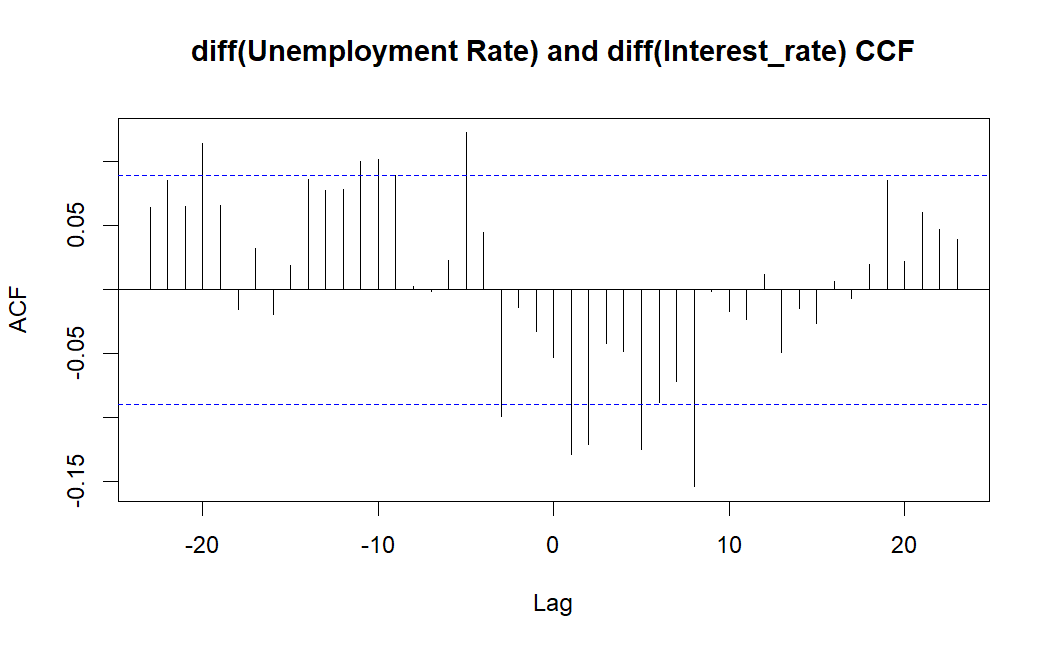
\includegraphics[width=10cm]{figs/ccf-UR-IR}
\caption{differenced UR and differenced IR cross-correlation}
\label{fig:ccf-UR-IR}
\end{figure}

\begin{figure}[H]
\centering
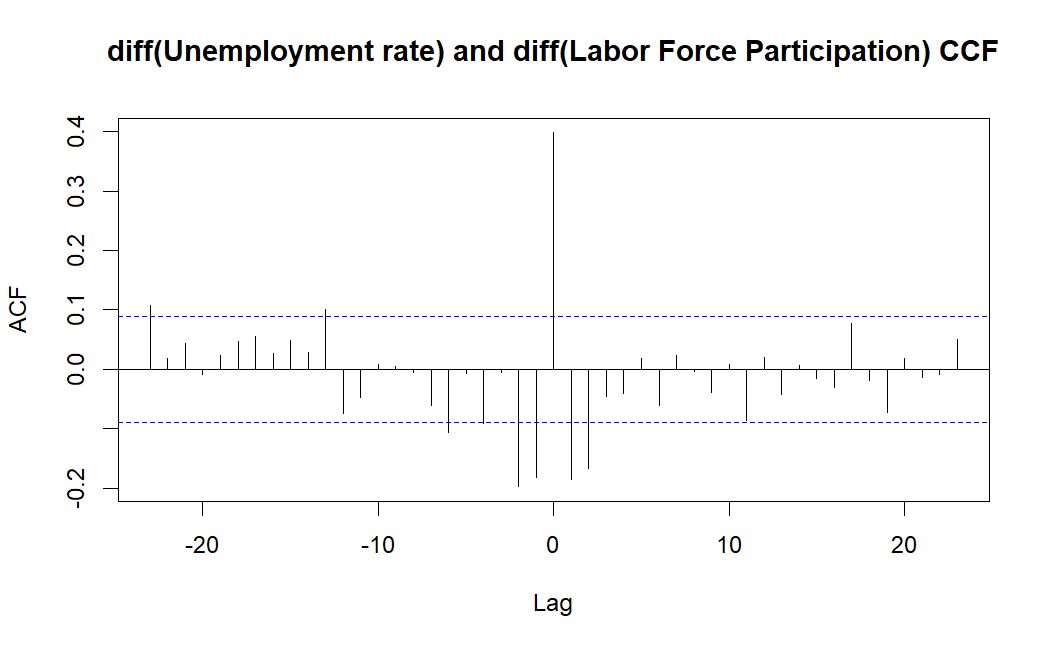
\includegraphics[width=10cm]{figs/ccf-UR-LFP}
\caption{differenced UR and differenced LFP cross-correlation}
\label{fig:ccf-UR-LFP}
\end{figure}

\begin{figure}[H]
\centering
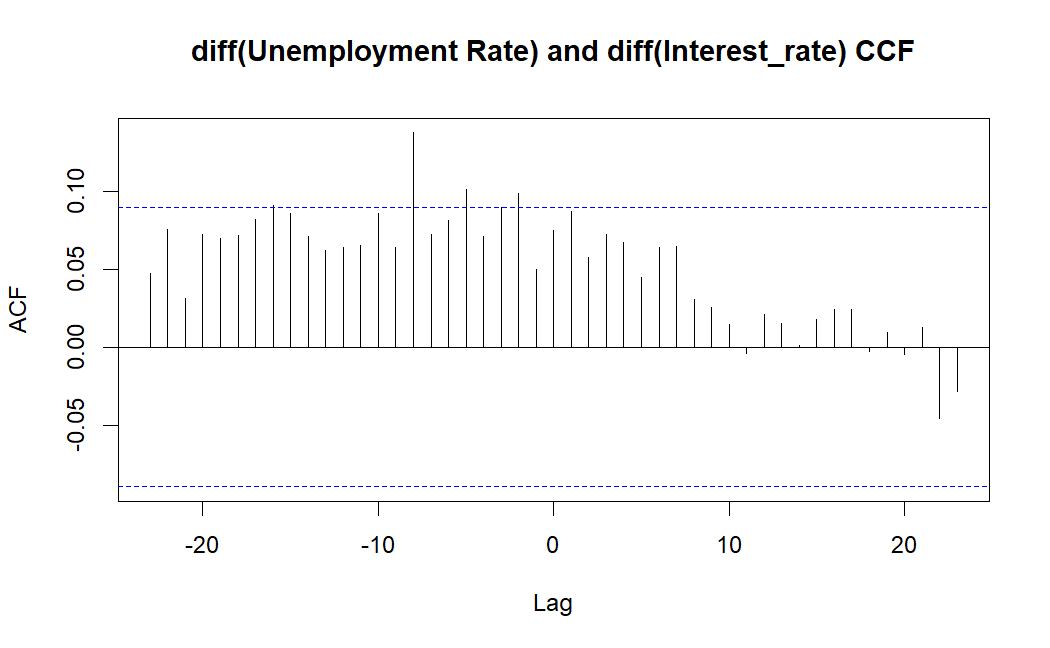
\includegraphics[width=10cm]{figs/ccf-UR-WAP}
\caption{differenced UR and differenced WAP cross-correlation}
\label{fig:ccf-UR-WAP}
\end{figure}

In \cref{fig:ccf-UR-LFP} we can see that unemployment rate is moderately correlated with LFP at lag 0, which indicates a potential predictor for forecasting unemployment rate.  \cref{fig:ccf-UR-WAP} also shows a slight correlation with unemployment rate at lag 8, but is excluded in the model for the reasons explained below. \cref{fig:ccf-UR-IR} also has a slight correlation with unemployment rate at lag 5, but is not as significant as the relationship between unemployment rate and LFP. 






\subsubsection*{Best ARMAX model based on Holdout RMSE}
Similar to the steps of the ARIMA model, our baseline ARIMAX model was produced from the \texttt{auto.arima()} function with xreg equal to our explanatory variables. WAP is excluded from our model as it had no significant contribution to the model in terms of forecasting abilities. The equations of the models with the best AIC and RMSE are provided below.  

TODO !!!
\begin{align}
 Y_t &= \\
 Y_t &= 
\end{align}

We then varied the p, q, P and Q values around the baseline model using \texttt{Arima()} and calculated the moving 1-step holdout set RMSE values.

\begin{table}[H]
    \centering
    \captionsetup{justification=centering,margin=2cm}
    \begin{tabular}{|c|c|c|}
    \hline
     Model & AIC & RMSE\\
    \hline\hline
    \textbf{best AIC:}(2,0,2)(1,0,0){[}12{]} & -304.56  & 3.723 \\
    \textbf{best RMSE:}
    (1,0,2)(1,0,0){[}12{]}             & -255.06  & 2.754 \\
    \hline
    (2,0,1)(1,0,0){[}12{]}             & -303.66  & 3.768 \\
    (2,1,2)(1,1,0){[}12{]}             & -37.06   & 3.546 \\
    (3,0,2)(1,0,0){[}12{]}             & -304.3   & 3.537 \\
    (2,0,2)(2,0,1){[}12{]}             & -249.57  & 3.332 \\
    (2,0,2)(2,0,0){[}12{]}             & -193.883 & 3.706 \\
    \hline
    \end{tabular}
    \caption{Summary of AIC and holdout RMSE values based on\\ 1-step forecasts for the baseline and perturbed models.
    }
    \label{table:armax-model}
\end{table}

Shown in \Cref{table:armax-model}, the model chosen by \texttt{auto.arima()} selected ARIMA$(2,0,2)(1,0,0)_12$ errors. Similar to the ARIMA models, this selected ARIMAX model is based on the lowest AIC values, rather than the one-step holdout RMSE. The model ARIMA$(1,0,2)(1,0,0)_12$ yields the lowest holdout RMSE value of 2.754. However, this value is high compared to the RMSE values of the seasonal persistence, average, Holt-Winters, and ARIMA forecasting methods. Therefore, this ARIMAX model is not our best choice as it does not have the best predictive accuracy. 

However, the above model ARIMA$(1,0,2)(1,0,0)_12$ with the Maximum Likelihood method outputs a holdout RMSE value of 0.994. This value is significantly lower than the 2.754 produced by the model using the default method. Comparing the RMSE values, this ML ARIMAX model has a better predictive accuracy than the seasonal persistence, average, and Holt-Winters forecasting methods.

\section{Contribution}

The team was divided into two groups based on availability and common interest in the research topic. Names are ordered in alphabetical order by surname. The major contributions for each subject are summarized in the table below

\begin{table}[H]
    \centering
    \captionsetup{justification=centering,margin=2cm}
    \begin{tabular}{|l|l|}
    \hline
        Topic & Names \\
    \hline\hline
    Persistence, Average, and Exp. Smoothing & Owen and Kaichi \\
    ARIMA and ARMAX & Lily, Sky, and Nico \\
    Writing & Lily, Sky, Nico, Owen, Kaichi \\
    \hline
   
    \end{tabular}
    \label{table:contribution}
\end{table}


\section{Appendix}

\subsection*{Data Sources}


\noindent
\textbf{Monthly Unemployment Rate (Age 15-64) Canada}\\
\indent
Organization for Economic Co-operation and Development, Infra-Annual Labor Statistics: Unemployment Rate Total: From 15 to 64 Years for Canada [LRUN64TTCAM156S], retrieved from FRED, Federal Reserve Bank of St. Louis; \url{https://fred.stlouisfed.org/series/LRUN64TTCAM156S}\\


\noindent
\textbf{Monthly Working-age Population (Age 15-64) Canada}\\
\indent 
Organization for Economic Co-operation and Development, Infra-Annual Labor Statistics: Working-Age Population Total: From 15 to 64 Years for Canada [LFWA64TTCAM647S], retrieved from FRED, Federal Reserve Bank of St. Louis; \url{https://fred.stlouisfed.org/series/LFWA64TTCAM647S}\\

\noindent
\textbf{Monthly Labour Force Participation Rate (Age 15-64) Canada}\\
\indent
Organization for Economic Co-operation and Development, Infra-Annual Labor Statistics: Labor Force Participation Rate Total: From 15 to 64 Years for Canada [LRAC64TTCAM156S], retrieved from FRED, Federal Reserve Bank of St. Louis; \url{https://fred.stlouisfed.org/series/LRAC64TTCAM156S}\\

\noindent
\textbf{Monthly Interest Rate Canada}\\
\indent
Organization for Economic Co-operation and Development, Interest Rates: Long-Term Government Bond Yields: 10-Year: Main (Including Benchmark) for Canada [IRLTLT01CAM156N], retrieved from FRED, Federal Reserve Bank of St. Louis; \url{https://fred.stlouisfed.org/series/IRLTLT01CAM156N}








\end{document}

